\documentclass{beamer}

% You can uncomment the themes below if you would like to use a different
% one:
%\usetheme{AnnArbor}
%\usetheme{Antibes}
%\usetheme{Bergen}
%\usetheme{Berkeley}
%\usetheme{Berlin}
%\usetheme{Boadilla}
%\usetheme{boxes}
%\usetheme{CambridgeUS}
%\usetheme{Copenhagen}
%\usetheme{Darmstadt}
%\usetheme{default}
%\usetheme{Frankfurt}
%\usetheme{Goettingen}
%\usetheme{Hannover}
%\usetheme{Ilmenau}
%\usetheme{JuanLesPins}
%\usetheme{Luebeck}
\usetheme{Madrid}
%\usetheme{Malmoe}
%\usetheme{Marburg}
%\usetheme{Montpellier}
%\usetheme{PaloAlto}
%\usetheme{Pittsburgh}
%\usetheme{Rochester}
%\usetheme{Singapore}
%\usetheme{Szeged}
%\usetheme{Warsaw}

\usepackage{cite}
\usepackage{amsmath,amssymb,amsfonts}

\usepackage{graphicx}
\usepackage{textcomp}
\usepackage{xcolor}
\usepackage{tikz}
\usepackage{verbatim}
\usepackage{algorithm}
\usepackage[noend]{algpseudocode}
\usepackage{multirow}
\usepackage{url}
%\usepackage[sorting=none]{biblatex}
\usepackage[utf8]{inputenc}
\usepackage{ifthen}
\usepackage{filecontents}
\usetikzlibrary{shapes,arrows,shadings,patterns}
\usepackage{pgfplots}
\pgfplotsset{compat=newest}
\pgfplotsset{plot coordinates/math parser=false}

\makeatletter
\def\BState{\State\hskip-\ALG@thistlm}
\makeatother

\usetikzlibrary{positioning}
\def\BibTeX{{\rm B\kern-.05em{\sc i\kern-.025em b}\kern-.08em
    T\kern-.1667em\lower.7ex\hbox{E}\kern-.125emX}}
    
\makeatletter
\def\endthebibliography{%
  \def\@noitemerr{\@latex@warning{Empty `thebibliography' environment}}%
  \endlist
}
\makeatother    
    
\makeatletter
\def\thickhline{%
  \noalign{\ifnum0=`}\fi\hrule \@height \thickarrayrulewidth \futurelet
   \reserved@a\@xthickhline}
\def\@xthickhline{\ifx\reserved@a\thickhline
               \vskip\doublerulesep
               \vskip-\thickarrayrulewidth
             \fi
      \ifnum0=`{\fi}}
\makeatother

\newlength{\thickarrayrulewidth}
\setlength{\thickarrayrulewidth}{3\arrayrulewidth}   


\title[Machine Learning and Communication]{Machine Learning Autoencoder Applied to Communication Channels}

\author{E.~Dadalto Camara Gomes\inst{1} \and M.~Benammar\inst{2}}
% - Give the names in the same order as the appear in the paper.
% - Use the \inst{?} command only if the authors have different
%   affiliation.

\institute[] % (optional, but mostly needed)
{
  \inst{1}%
   ISAE-SUPAERO\\
   Université de Toulouse\\
    31055, Toulouse, France\\
Email: eduardo.dadalto-camara-gomes@student.isae-supaero.fr
  \and
  \inst{2}%
  Department of Electronics, Optronics, and Signal processing\\
  ISAE-SUPAERO\\
  31055, Toulouse, France\\
  Email: meryem.benammar@isae-supaero.fr}
% - Use the \inst command only if there are several affiliations.
% - Keep it simple, no one is interested in your street address.

\date{ISAE-SUPAERO, 2019}
% - Either use conference name or its abbreviation.
% - Not really informative to the audience, more for people (including
%   yourself) who are reading the slides online

\subject{Machine Learning and Communication}
% This is only inserted into the PDF information catalog. Can be left
% out. 

% If you have a file called "university-logo-filename.xxx", where xxx
% is a graphic format that can be processed by latex or pdflatex,
% resp., then you can add a logo as follows:

%\pgfdeclareimage[height=0.5cm]{university-logo}{images/ISAE}
%\logo{\pgfuseimage{university-logo}}

% Delete this, if you do not want the table of contents to pop up at
% the beginning of each subsection:
%\AtBeginSubsection[]
%{
%  \begin{frame}<beamer>{Outline}
%    \tableofcontents[currentsection,currentsubsection]
%  \end{frame}
%}

% Let's get started
\begin{document}

\begin{frame}
  \titlepage
\end{frame}

\begin{frame}{Outline}
  \tableofcontents
  % You might wish to add the option [pausesections]
\end{frame}

% Section and subsections will appear in the presentation overview
% and table of contents.
\section{Introduction}

\begin{frame}{Context}{Communication system context in general - what field will I be treating}
  \begin{itemize}
  \item {
    My first point.
  }
  \item {
    My second point.
  }
  \end{itemize}
\end{frame}


\begin{frame}{Context}{Machine Learning applications - what could we do in communication system}
  \begin{itemize}
  \item {
    My first point.
  }
  \item {
    My second point.
  }
  \end{itemize}
\end{frame}

\begin{frame}{Relevance \& Challenges}{Explain why the work is relevant and explain what are the challenges}
  \begin{itemize}
  \item {
    My first point.
  }
  \item {
    My second point.
  }
  \end{itemize}
\end{frame}

\begin{frame}{Problem Statement}{What exactly I will solve in this work}
  \begin{itemize}
  \item {
    My first point.
  }
  \item {
    My second point.
  }
  \end{itemize}
\end{frame}


% You can reveal the parts of a slide one at a time
% with the \pause command:
\begin{frame}{Second Slide Title}
  \begin{itemize}
  \item {
    First item.
    \pause % The slide will pause after showing the first item
  }
  \item {   
    Second item.
  }
  % You can also specify when the content should appear
  % by using <n->:
  \item<3-> {
    Third item.
  }
  \item<4-> {
    Fourth item.
  }
  % or you can use the \uncover command to reveal general
  % content (not just \items):
  \item<5-> {
    Fifth item. \uncover<6->{Extra text in the fifth item.}
  }
  \end{itemize}
\end{frame}


\section{Methodology}

\subsection{Reference Model}
\begin{frame}{Maximum a Posterior (MAP) Rule}{Implementation of a MAP decoder for a linear block code through a BSC.}

 \begin{figure}[!ht]
  \centering
    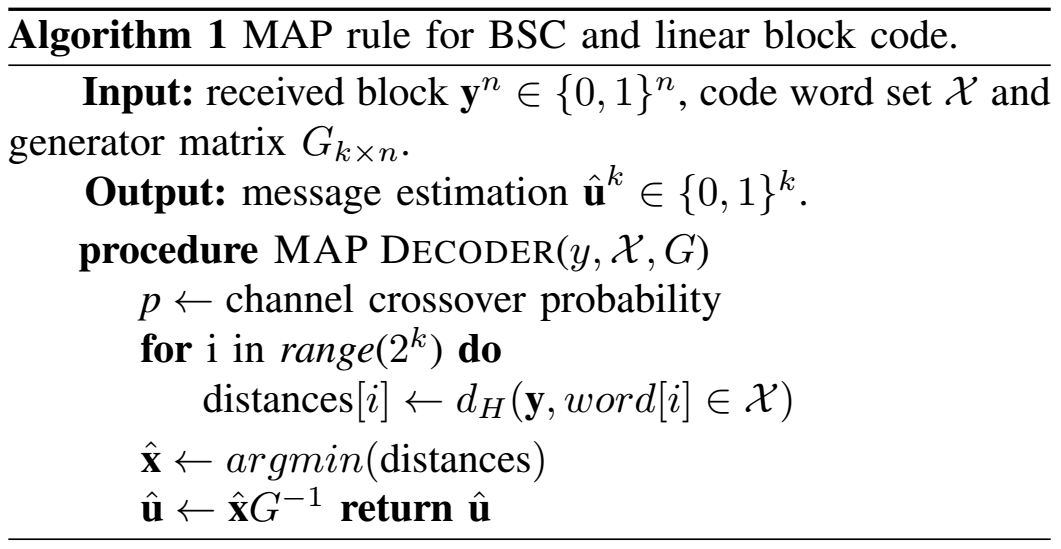
\includegraphics[width=0.8\textwidth]{images/algorithm}
\end{figure}

\end{frame}

\subsection{Design \& Architecture}
\begin{frame}[allowframebreaks]{Neural Network's Design and Architecture}{Show the architecture used for each case and remarks some important parameters}

	\begin{figure}[!ht]
  \centering
    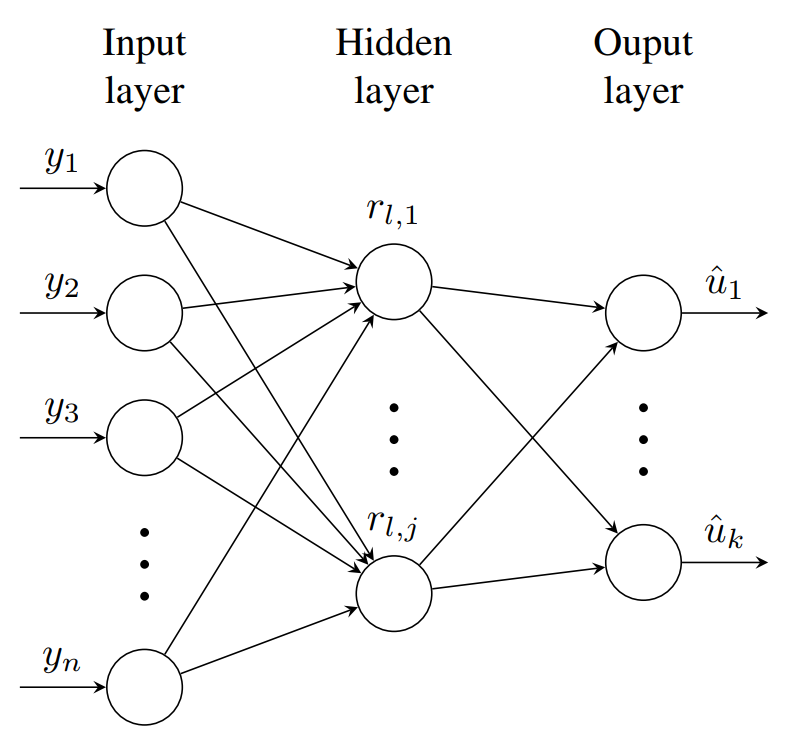
\includegraphics[width=0.4\textwidth]{images/MLNN}
    \caption{MLNN representative diagram, where $\textbf{y}^n$ is the input vector, $\textbf{r}_{l}^{j}$ is a hidden layer vector
and $\hat{\textbf{u}}^{k}$ is the output vector.} \label{fig:NN}
\end{figure}

	\framebreak

    \begin{table}
\caption{DNN array decoder architecture and parameters.} 
\begin{center}

  \begin{tabular}{ l  |  l }
    \thickhline
    \multirow{3}{*}{Decoder} & Dense: 128, activation: ReLU, input size: $n$ \\
 & Dense: 64, activation: ReLU  \\
 & Dense: 32, activation: ReLU  \\
 & Dense: $k$, activation: Sigmoid  \\ \hline
    \multicolumn{2}{l}{\textbf{Total parameters: $12776$}}\\
    \thickhline
  \end{tabular}
    \label{tab:arraydecoder}
\end{center}
\end{table}

\begin{center}
\begin{tabular}{ l  |  l | l | l  }
    \thickhline
 Loss func. & Optimizer & N. Epochs & Batch Size \\ \hline
 Binary cross-entropy & Adam & $2^{16}$ & $256$ \\
    \thickhline
  \end{tabular}
    \label{tab:arraydecoderTrain}
\end{center}

  \framebreak
 
    \begin{table}
\caption{DNN one-hot decoder architecture and parameters.} 
\begin{center}

  \begin{tabular}{ l  |  l }
    \thickhline
    \multirow{1}{*}{Decoder} & Dense: 256, activation: Softmax, input size: $n$ \\ \hline
    \multicolumn{2}{l}{\textbf{Total parameters: }$4352$}\\
    \thickhline
  \end{tabular}
    \label{tab:onehotdecoder}
\end{center}
\end{table}

\begin{center}
\begin{tabular}{ l  |  l | l | l  }
    \thickhline
 Loss func. & Optimizer & N. Epochs & Batch Size \\ \hline
 Binary cross-entropy & Adam & $2^{14}$ & $256$ \\
    \thickhline
  \end{tabular}
    \label{tab:onehotdecoderTrain}
\end{center}

	\framebreak
	
	\begin{figure}[!ht]
  \centering
    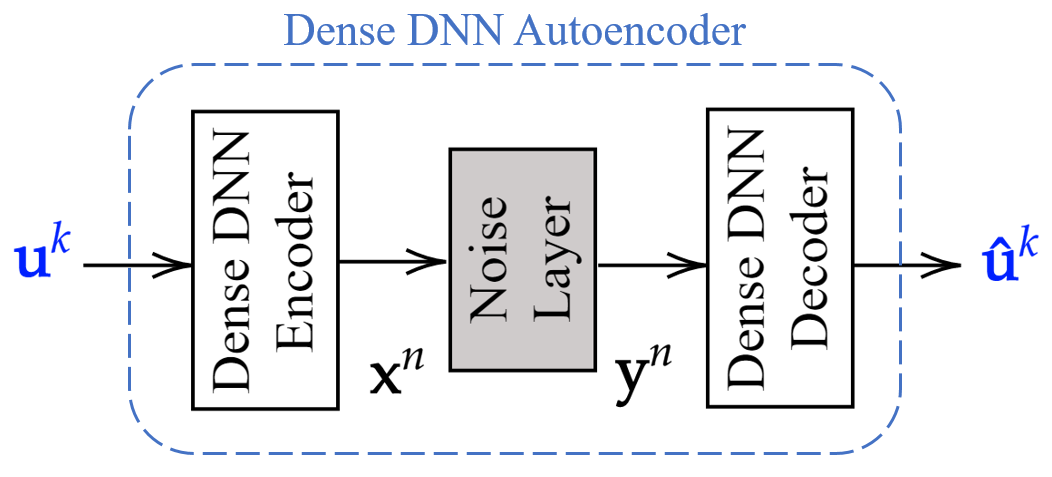
\includegraphics[width=0.8\textwidth]{images/DNN_autoencoder}
    \caption{Representation of a DNN autoencoder composed of dense layers.}\label{fig:DDNNAutoencoder}
\end{figure}
	
	\framebreak

    \begin{table}
\caption{DNN array autoencoder architecture.} 
\begin{center}
  \begin{tabular}{ l  |  l }
    \thickhline
    \multirow{3}{*}{Encoder} & Dense: 512, activation: ReLU, BN\footnotemark, input size: 8 \\
 & Dense: 256, activation: ReLU, BN \\
 & Dense: 16, activation: Sigmoid  \\ \hline
    \multirow{2}{*}{Channel} & Lambda: $Round(\textbf{x})$, input size: $16$ \\
 & Lambda: $\textbf{x}\oplus \text{noise}$\\ \hline
 \multirow{2}{*}{Decoder} & Dense: 128, BN, input size: 16 \\
 & Dense: 64, activation: ReLU, BN  \\
 & Dense: 8, activation: Sigmoid  \\ \hline
    \multicolumn{2}{l}{\textbf{Total parameters: }154072}\\
    \thickhline
  \end{tabular}
    \label{tab:arrayautoencoder}
\end{center}
\end{table}

\begin{center}
\begin{tabular}{ l  |  l | l | l  }
    \thickhline
 Loss func. & Optimizer & N. Epochs & Batch Size \\ \hline
 MSE & Adam & $2^{17}$ & $256$ \\
    \thickhline
  \end{tabular}
    \label{tab:arrayautoencoderTrain}
\end{center}

\footnotetext{Batch Normalization (BN)}

	\framebreak
  
    \begin{table}
\caption{DNN one-hot autoencoder architecture.} 
\begin{center}

  \begin{tabular}{ l  |  l }
    \thickhline
    \multirow{3}{*}{Encoder} & Dense: 196, activation: ReLU, BN, input size: 256\\
 & Dense: 128, activation: ReLU, BN  \\
 & Dense: 96, activation: ReLU, BN \\
 & Dense: 64, activation: ReLU, BN  \\
 & Dense: 32, activation: ReLU, BN  \\
 & Dense: 16, activation: Sigmoid  \\ \hline
   Channel & Lambda: $Round(\textbf{x})$, input size: $16$ \\ \hline
 Decoder & Dense: 128, activation: ReLU, BN, input size: 16 \\
 & Dense: 256, activation: Softmax  \\ \hline
    \multicolumn{2}{l}{\textbf{Total parameters: }134052}\\
    \thickhline
  \end{tabular}
    \label{tab:onehotautoencoder}
\end{center}
\end{table}

\begin{center}
\begin{tabular}{ l  |  l | l | l  }
    \thickhline
 Loss func. & Optimizer & N. Epochs & Batch Size \\ \hline
 MSE & Adam & $2^{16}$ & $256$ \\
    \thickhline
  \end{tabular}
    \label{tab:onehotautoencoderTrain}
\end{center}


\end{frame}


\subsection{Error Correction \& Predictions}
\begin{frame}{Error Correction and Monte Carlo Simulations}{Explain how we could use NN to predict the results with certain confidence.}
  \begin{itemize}
  \item {
    My first point.
  }
  \item {
    My second point.
  }
  \end{itemize}
\end{frame}


\begin{frame}{Blocks}
\begin{block}{Block Title}
You can also highlight sections of your presentation in a block, with it's own title
\end{block}
\begin{theorem}
There are separate environments for theorems, examples, definitions and proofs.
\end{theorem}
\begin{example}
Here is an example of an example block.
\end{example}
\end{frame}

% Placing a * after \section means it will not show in the
% outline or table of contents.

\section{Results \& Discussions}
\subsection{DNN Decoders}
\begin{frame}{DNN Array Decoder}{Show the results for the array decoder in terms of train p, Mep, Parameters, etc}
 
 \begin{figure}[!ht]
  \centering
    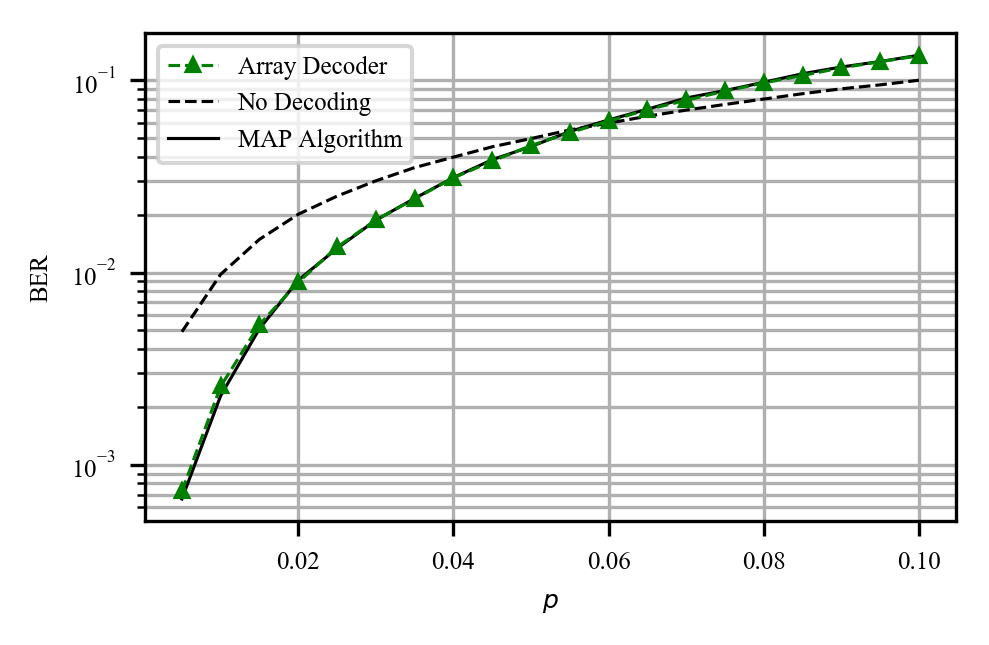
\includegraphics[width=0.8\textwidth]{images/MLNN_Mep_65536_ptrain_007}
    \caption{Array decoding BER performance. NN trained with a channel crossover probability error of $p_t=0.07$.}\label{fig:ArrayD}
\end{figure}
 

\end{frame}

\begin{frame}{DNN One-hot Decoder}{Show the results for the one-hot decoder in terms of train p, Mep, Parameters, etc}
    
   \begin{figure}[!ht]
  \centering
    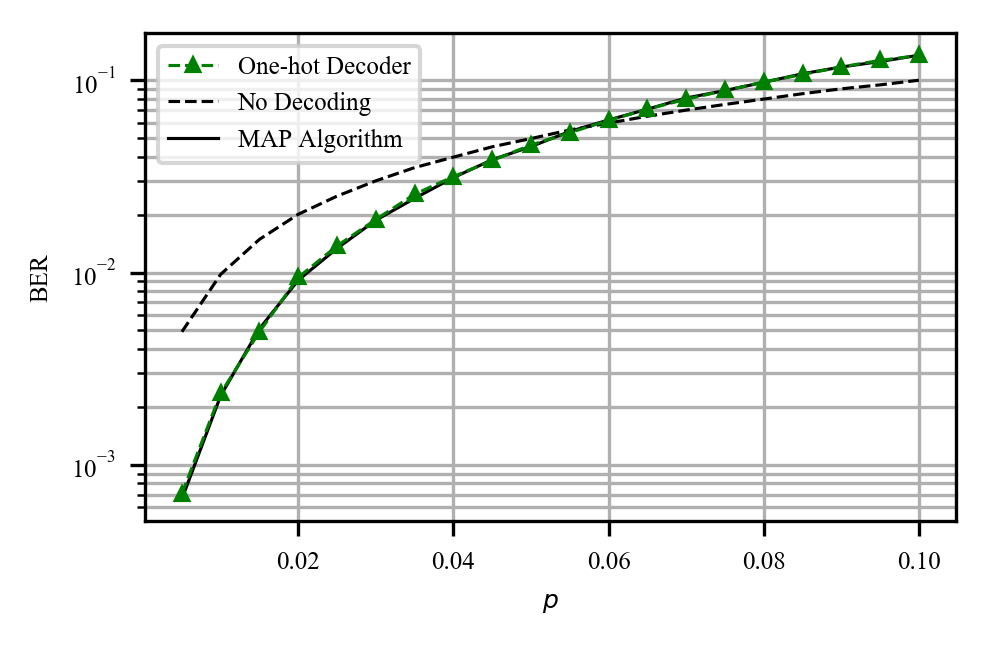
\includegraphics[width=0.8\textwidth]{images/MLNN1H_Mep_16384_ptrain_0}
    \caption{One hot decoding BER performance. NN decoder trained with a channel crossover probability error of $p_t=0$.}\label{fig:1HD}
\end{figure}

\end{frame}

\subsection{DNN Autoencoders}
\begin{frame}[allowframebreaks]{DNN Array Autoencoder}{Show the results for the autoencoder in terms of train p, Mep, Parameters, etc}

\begin{figure}[!ht]
  \centering
    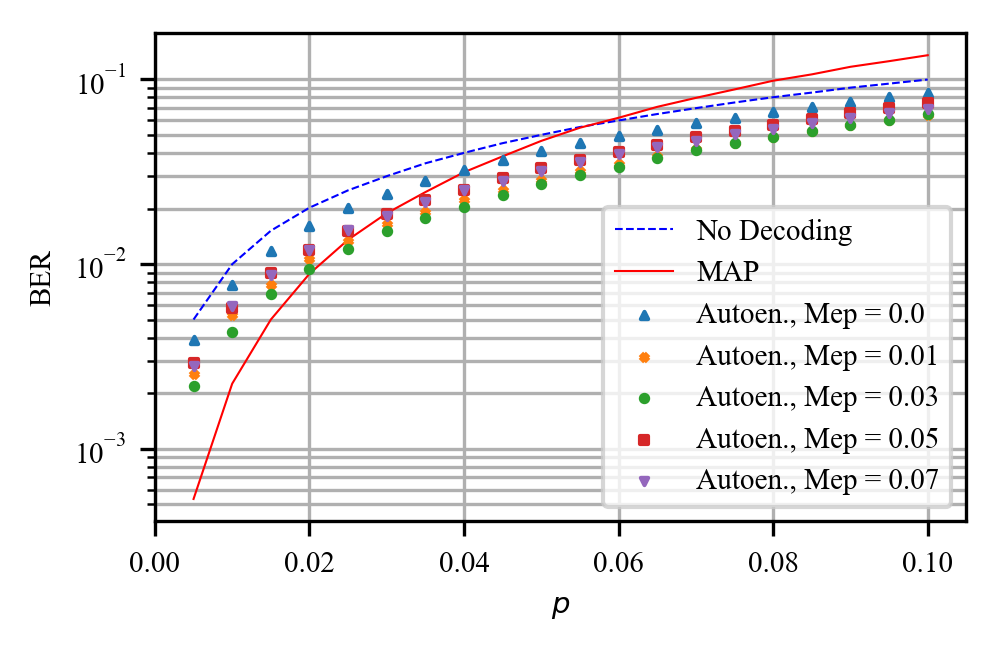
\includegraphics[width=0.8\textwidth]{images/MAP_AutoencoderArray_Mep_65536_64_128_256_p_analysis}
    \caption{Training crossover probability simulation for the array autoencoder. $P_t=0.3$ demonstrated to have best performance to this particular architecture.}\label{fig:parrayanalysis}
\end{figure}


\begin{figure}[!ht]
  \centering
    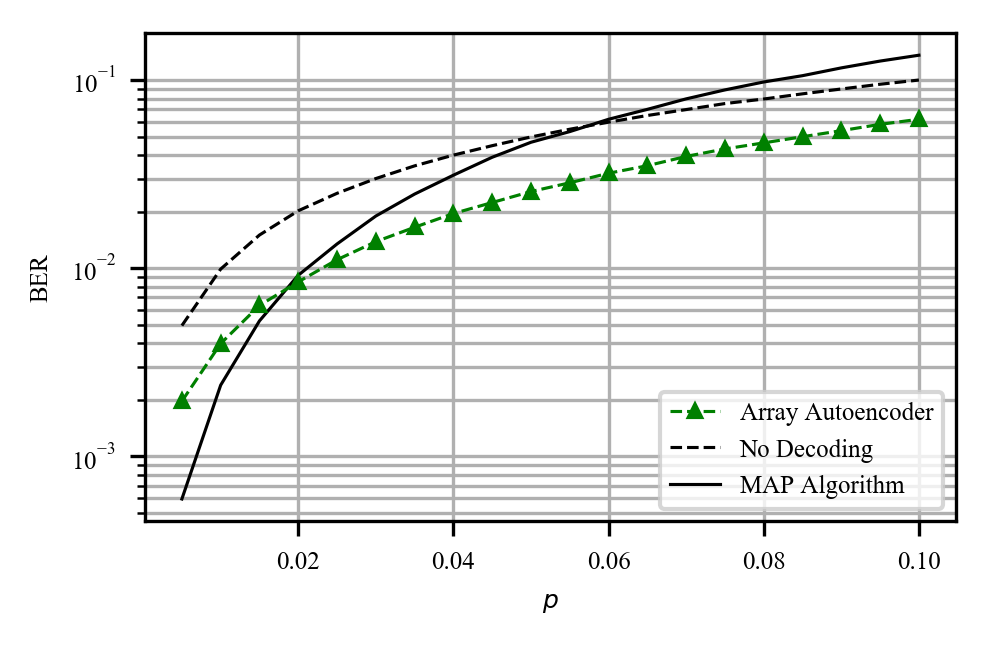
\includegraphics[width=0.8\textwidth]{images/AutoencoderArray_Mep_65536_ptrain_003_logcosh}
    \caption{Array autoencoder BER performance. DNN array autoencoder trained with a channel crossover probability error of $p_t=0.03$.}\label{fig:arrayautoencoder}
\end{figure}

\end{frame}

\begin{frame}{DNN One-hot Autoencoder}{Show the results for the autoencoder in terms of train p, Mep, Parameters, etc}

\begin{figure}[!ht]
  \centering
    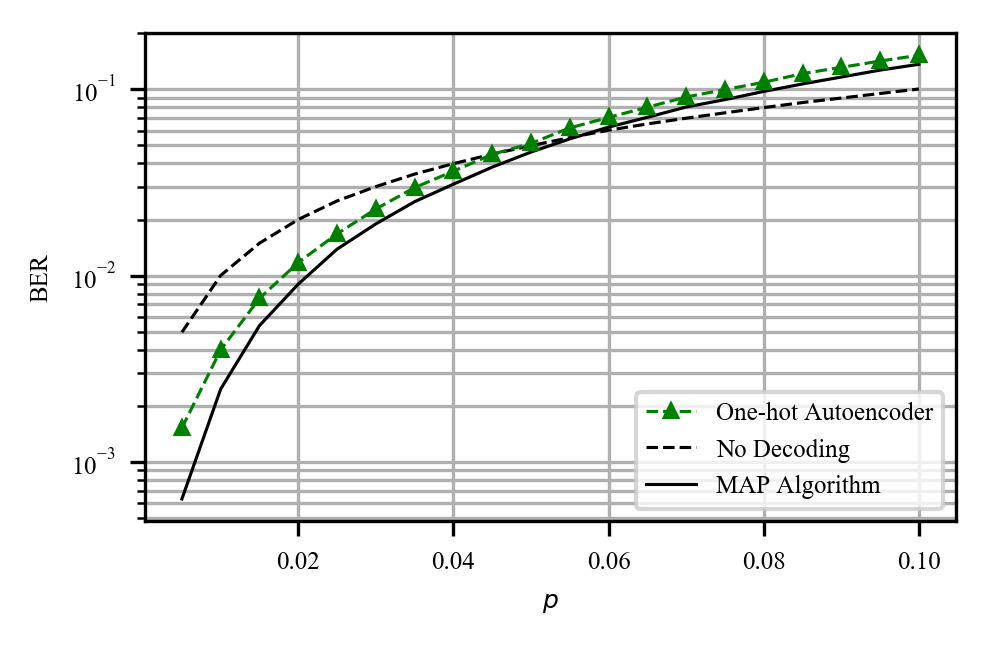
\includegraphics[width=0.75\textwidth]{images/MAP_Autoencoder1H_Mep_131072_ptrain_0_192_128_96_64_32-128}
    \caption{One-hot autoencdoer BER performance. Trained without a noisy channel.}\label{fig:1hautoencoder}
\end{figure}

\end{frame}



\subsection{Time Analysis}
\begin{frame}{Delay Time Analysis}{Comparison of encoding, transmission and decoding time for each method.}
  \begin{table}
\caption{Decoding time comparison between the MAP algorithm and the DNN decoders and autoencoders. The data is normalized to the average MAP algorithm decoding time. } 
\begin{center}

  \begin{tabular}{ c | c | c}
    \thickhline
    MAP & Array Decoder & One-hot Decoder\\
    $1.00 \pm 0.02$ & $0.74 \pm 0.03$ & $0.76 \pm 0.02$ \\ \hline
    \multicolumn{2}{c|}{Array Autoencoder}  & One-hot Autoencoder\\
   
     \multicolumn{2}{c|}{$1.33 \pm 0.05 $} & $3.02 \pm 0.06$ \\ 
    \thickhline
  \end{tabular}
    \label{tab:timeanalysis}
\end{center}
\end{table}

\end{frame}

\section{Conclusions}
\begin{frame}{Conclusions}
  \begin{itemize}
  \item {
    My first point.
  }
  \item {
    My second point.
  }
  \end{itemize}
\end{frame}

\section{Future Work}
\begin{frame}{Future Work}
  \begin{itemize}
  \item {
    My first point.
  }
  \item {
    My second point.
  }
  \end{itemize}
\end{frame}

\section*{Acknowledgment}

\begin{frame}{Acknowledgment}
  I would like to thank ...
  \begin{itemize}
   \item{The guidance and advice from my supervisor Meryem Benammar, Ph.D;}
  \item{ My colleague Rémy Zawislak who worked in the same theme and collaborated indirectly to the research;}
   \item{Marjorie Grzeskowiak Lucas, Ph.D, who through the Institut Supérieur de l'Aéronautique et de l'Espace (ISAE-SUPAERO) enabled the confection of the project; and }
   \item{The supervisors, the LACS member and the audience present today.}
  \end{itemize}

 
\end{frame}

\appendix
\section<presentation>*{Bibliography}

\begin{frame}[allowframebreaks]
  \frametitle<presentation>{Bibliography}
    

\color{white}
\cite{Shannon:2001:MTC:584091.584093, DBLP:journals/corr/CalabreseWGPS16, DBLP:journals/corr/OSheaH17, 2016arXiv160806409O, 2017arXiv171008379G, Worm00turbo-decodingwithout, Viterbi, journals/ett/RobertsonHV97, HagenauerJ, JordanMA,Ibnkahla, nielsenneural, murphy2013machine, DBLP:journals/corr/AbadiABBCCCDDDG16, chollet2015keras, doi:10.1162/neco.2006.18.7.1527, DBLP:conf/acssc/BenammarP18, DBLP:journals/corr/KeskarMNST16, DBLP:journals/corr/IoffeS15}

\bibliographystyle{ieeetr}
\bibliography{bib/ShannonCE1948,bib/CalabreseWGPS16,bib/OSheaH17,bib/Oshea2,bib/Gruber,bib/Worm,bib/Viterbi,bib/RobertsonHV97,bib/HagenauerJ,bib/JordanMA,bib/Ibnkahla,bib/Nielsen,bib/Murphy,bib/AbadiABBCCCDDDG16,bib/Keras,bib/mit_neco18_1527,bib/BenammarP18,bib/KeskarMNST16,bib/IoffeS15}
 
\end{frame}

\end{document}


